% Research paper (Introduction, Methodology, Results, Discussion) on the two main findings of the project
% "Accelerating Variance Reduction" and its side study on Muon: (1) certified rates lose at the global constants and no
% fixed geometry repairs the worst case, for SAGA as for Muon-type (polar) steps; (2) through the polar map, variance
% reduction acts on the fixed point of the method (the nuclear median of the noise), not only on a variance term.
% Sources: report/main.pdf (main report), muon/findings.md + muon/results/digest.md (experiments on Muon),
% muon/notes_spectral_theory.pdf and muon/notes_theory.md (theory, proofs); the extended report
% muon/report_spectral_muon_new.pdf covers the other results.
% Build (from muon/):  pdflatex paper_saga_to_muon && bibtex paper_saga_to_muon && pdflatex paper_saga_to_muon && pdflatex paper_saga_to_muon
% Figures: muon/report_figures/make_figR1_classical.py, make_figP2_geometry.py, make_figP3_noise.py.
% Bibliography: paper_saga_to_muon.bib, generated by
%   _scratch/muon_checks/make_report_bib.py muon/paper_saga_to_muon.tex --out muon/paper_saga_to_muon.bib
\documentclass[10pt]{article}
\usepackage[utf8]{inputenc}
\usepackage[T1]{fontenc}
\usepackage{amsmath,amssymb,amsthm,mathtools}
\usepackage{graphicx}
\usepackage{booktabs}
\usepackage{tabularx}
\usepackage{array}
\usepackage{enumitem}
\usepackage{multicol}
\usepackage{etoolbox}
\usepackage[margin=1in]{geometry}
\usepackage[colorlinks=true,linkcolor=blue!55!black,citecolor=blue!55!black,urlcolor=blue!55!black]{hyperref}
\usepackage{xcolor}
\graphicspath{{figures/}}
\setlength{\emergencystretch}{2em}
\clubpenalty=10000 \widowpenalty=10000
\setlength{\textfloatsep}{10pt plus 2pt minus 2pt}
\setlength{\abovecaptionskip}{4pt}
\renewcommand{\topfraction}{0.9}
\renewcommand{\bottomfraction}{0.6}
\renewcommand{\textfraction}{0.08}
\renewcommand{\floatpagefraction}{0.8}
\setcounter{topnumber}{2}
\setcounter{totalnumber}{3}
% compact headings
\makeatletter
\renewcommand\section{\@startsection{section}{1}{\z@}{-2.4ex \@plus -0.6ex \@minus -.2ex}{1.2ex \@plus .2ex}{\normalfont\large\bfseries}}
\renewcommand\subsection{\@startsection{subsection}{2}{\z@}{-1.8ex\@plus -0.5ex \@minus -.2ex}{0.8ex \@plus .2ex}{\normalfont\normalsize\bfseries}}
\makeatother

\newtheorem{theorem}{Theorem}
\newtheorem{proposition}[theorem]{Proposition}
\theoremstyle{remark}
\newtheorem*{remark}{Remark}

\newcommand{\R}{\mathbb{R}}
\newcommand{\E}{\mathbb{E}}
\newcommand{\Prob}{\mathbb{P}}
\newcommand{\norm}[1]{\left\|#1\right\|}
\newcommand{\nop}[1]{\left\|#1\right\|_{\mathrm{op}}}
\newcommand{\nnuc}[1]{\left\|#1\right\|_{*}}
\newcommand{\nF}[1]{\left\|#1\right\|_{F}}
\newcommand{\inner}[2]{\left\langle #1, #2 \right\rangle}
\newcommand{\abs}[1]{\left|#1\right|}
\newcommand{\tr}{\operatorname{tr}}
\newcommand{\diag}{\operatorname{diag}}
\newcommand{\polar}{\operatorname{polar}}
\newcommand{\Med}{\operatorname{Med}_\ast}
\newcommand{\Lop}{L_{\mathrm{op}}}
\newcommand{\muop}{\mu_{\mathrm{op}}}
\newcommand{\kop}{\kappa_{\mathrm{op}}}
\newcommand{\kF}{\kappa_{F}}
\newcommand{\lmin}{\lambda_{\min}}
\newcommand{\lmax}{\lambda_{\max}}
\newcommand{\ones}{\mathbf{1}}
\newcommand{\etas}{\eta_\ast}
\newcommand{\muEff}{\mu_{\mathrm{eff}}}
\newcommand{\LEff}{L_{\mathrm{eff}}}
\newcommand{\muPL}{\mu_{\mathrm{PL}}}
\newcommand{\finding}[1]{\textbf{(#1)}}
\newcommand{\nat}[1]{\textsc{[#1]}}
\newcolumntype{Y}{>{\raggedright\arraybackslash}X}

% compact two-column bibliography (the heading is set by the multicols environment)
\patchcmd{\thebibliography}{\section*{\refname}}{}{}{\typeout{PATCH OF THEBIBLIOGRAPHY FAILED}}
\let\oldthebibliography\thebibliography
\renewcommand{\thebibliography}[1]{\oldthebibliography{#1}\setlength{\itemsep}{0.5pt}\setlength{\parskip}{0pt}}

\title{\vspace{-2.2em}From SAGA to Muon-type steps:\\ no norm repairs the logistic worst case, and variance reduction
acts on the fixed point}
\author{Project ``Accelerating Variance Reduction'' and its side study on Muon\\ Statistical Learning Theory, UC Berkeley}
\date{\vspace{-0.4em}17 November 2026}

\begin{document}
\maketitle

\begin{abstract}
The linear rate of SAGA rests on a geometry, global constants that certify the decrease of a Lyapunov function, and on
an estimator, unbiased and with an error that vanishes at the minimizer. Muon-type steps, along the polar factor of a
matrix gradient, change both. We follow each property from SAGA to such steps. \emph{Finding 1: certified rates lose at
the global constants, and no fixed norm repairs the logistic worst case.} Measured exactly along runs on ridge logistic
regression, the exact contraction exponent of SAGA is $3.2$ to $220$ times the certified one, and for $\kappa\ge10^4$,
$77$--$96\%$ of the gap comes from the two inequalities that replace the curvature met along the run, up to $81$ times
the global constant, by global constants; the exact one-step formula of the nuclear-scaled polar step on quadratics has
the same anatomy. Yet for ridge-regularized generalized linear models whose loss curvature vanishes along a sequence, no
norm, the spectral one included, has a better worst-case condition number than the Euclidean one; on a tuned benchmark,
Euclidean devices match the gain of orthogonalization over SAGA. \emph{Finding 2: through the polar map, variance
reduction acts on the fixed point.} With additive gradient noise and suitably decreasing deterministic lengths, stochastic polar steps
on smooth strongly convex objectives are stochastic mirror descent on a noise-smoothed nuclear norm and converge almost
surely to a point where the gradient is minus a \emph{nuclear median} of the noise, an offset formally of order $1/b$
for minibatches with skewed entries; a finite-sum estimator makes the minimizer the only fixed point and, with a step
that vanishes with it, reaches rounding precision in experiments. We propose no method that beats the state of the art.
\end{abstract}

\section{Introduction}\label{sec:intro}

\paragraph{Context.} For a finite sum $F=\frac1n\sum_if_i$, variance-reduced methods such as SVRG
\cite{johnson2013accelerating} and SAGA \cite{defazio2014saga} converge linearly with a constant step. Proposition~5.9 of \cite{bach2024learning} proves it for SAGA with
a Lyapunov function and global constants; accelerated variants reach the optimal order
$(n+\sqrt{n\kappa})\log(1/\varepsilon)$ \cite{allenzhu2018katyusha,kovalev2020dont,lan2018optimal}. Muon
\cite{jordan2024muon} steps along an approximation (by Newton--Schulz iterations) of the polar factor of the momentum of
the gradient of each weight matrix; without momentum this is steepest descent for the spectral norm
\cite{carlson2015stochastic,bernstein2024old}. Its theory is recent: the dynamics on least squares
\cite{shulgin2026quadratic,vasudeva2025muon} and the effect of gradient noise \cite{xie2026muon,chen2026when,paquette2026phases}
are being worked out, and its published variance-reduced versions are mostly momentum-based \cite{liu2025marsm}.

\paragraph{Question and findings.} The guarantee of SAGA rests on two properties: a \emph{geometry}, in which global
constants $R^2$ and $\mu$ certify that a Lyapunov function contracts, and an \emph{estimator}, unbiased (in a linear
step the mean step is the gradient step) and with an error that vanishes at the minimizer (which removes the variance
term). A Muon-type step changes both: it measures steps in the spectral norm and applies a nonlinear map, the polar
factor, to the estimator. We follow each property, treating proofs as measurable objects
(conditional expectations along runs are computed exactly). \emph{(1) Geometry:} certified rates lose
where global constants replace the curvature met along the run (measured for SAGA, by an exact formula for the polar
step), but for ridge
models with vanishing loss curvature no norm improves the worst case (Theorem~\ref{thm:nfl}); there a change of
norm, Muon's included, can only buy properties of trajectories, which Euclidean devices reproduce on our benchmark. \emph{(2) Estimator:}
through the polar map unbiasedness is lost, and, with additive noise and deterministic decreasing lengths, polar steps
converge to a point where the gradient is minus a
nuclear median of the noise (Theorem~\ref{thm:smd}); the vanishing error survives, and a finite-sum estimator makes the
minimizer the only fixed point (Proposition~\ref{prop:comp}(c)): inside polar steps, variance reduction buys precision
more than speed.

\paragraph{Contributions.} Table~\ref{tab:sota} sets each result against the published state of the art (we propose no
method that beats it) and Table~\ref{tab:link} sums up the link from SAGA to Muon-type steps. Other results, the proofs
and the numbers are in the main report, the extended report, the theory notes and the logs (files listed at the end).

\begin{table}[t]
\caption{What was published and what this study adds. Tags (Section~\ref{sec:status}): \nat{p} proved, \nat{m}
measured exactly along runs, \nat{e} experiment, \nat{f} formal expansion checked by simulation. The additions were not
found by the literature checks of Section~\ref{sec:status}, with the exceptions listed there.}\label{tab:sota}
\centering\footnotesize
\renewcommand{\arraystretch}{1.1}
\begin{tabularx}{\textwidth}{@{}>{\raggedright\arraybackslash}p{0.15\textwidth}YY@{}}
\toprule
Question & Published state of the art & Added by this study \\
\midrule
Where does the proof of SAGA lose? \finding{C1}--\finding{C3} &
Rate and Lyapunov proof \cite{defazio2014saga,bach2024learning}; worst case over a class of functions by performance
estimation and matrix inequalities \cite{taylor2017smooth,hu2017unified}; one-point curvature conditions
\cite{zhang2013gradient}; exact one-step formula of the nuclear-scaled step on least squares, its tight worst case
and its dependence on the trajectory \cite{shulgin2026quadratic,jawanpuria2026constant}. &
Each inequality of the proof evaluated along runs \nat{m}: exact exponent $3.2$--$220$ times the certified
one; $77$--$96\%$ of the gap due to the two global constants ($\kappa\ge10^4$); curvature met up to
$81\mu$. The same anatomy for the polar step \nat{p}. \\
Can a change of geometry improve the worst case? \finding{C5}, Thm.~\ref{thm:nfl}, \finding{M3}, \finding{M4} &
SAGA in a fixed metric \cite{dragomir2021fast,kolte2015accelerating}; preconditioning helps where the loss curvature
is bounded below (square loss; logistic loss on bounded sets) \cite{yang2014data,gonen2016solving}, and no linear
preconditioner helps some functions \cite{hird2025quantifying}; Muon as spectral steepest descent
\cite{bernstein2024old}. &
When the loss curvature vanishes along a sequence (logistic, softmax), no fixed preconditioner and no norm improves the
global or per-sample condition numbers \nat{p}; on least squares, a polar metric frozen at $W_0$ improves the latter
\nat{e}; tuned Euclidean devices match orthogonalization \nat{e}. \\
What does gradient noise do to a polar step? Thm.~\ref{thm:smd}, Props.~\ref{prop:comp}--\ref{prop:offset} &
Noise smooths the polar map \cite{xie2026muon,chen2026when}; sign methods follow a median and converge under
unimodal symmetric noise \cite{chen2020distributed,bernstein2019majority}; normalized steps estimate the geometric
median \cite{cardot2013efficient} and, under symmetric noise densities, converge \cite{jakovetic2023nonlinear}; in dimension one Muon need not converge under skewed noise \cite{do2026muon}. &
With additive noise, polar steps are stochastic mirror descent on a smoothed nuclear norm and, for deterministic decreasing lengths,
converge to a point where the gradient is minus a nuclear median of the noise \nat{p}; at batch one on least squares
($K,d\ge2$), to a least-distances estimator \nat{p}; for i.i.d.\ skewed entries, a limit gradient of order $1/b$, per
entry a factor of order $\max(K,d)$ below sign descent \nat{f}. \\
What does a finite-sum estimator change? Prop.~\ref{prop:comp}(c), \finding{M1}, \finding{M2} &
Momentum-based variance reduction for Muon \cite{liu2025marsm}; SVRG in a fixed-length polar step,
restoring the full-batch limit direction on separable data \cite{li2026implicit}, and in sign descent \cite{chzhen2023signsvrg}; floors of fixed lengths
\cite{lau2025polargrad,jawanpuria2026constant}; MISO \cite{mairal2015incremental}. &
The minimizer becomes the only fixed point \nat{p}; rounding precision needs a step that vanishes with the estimator
\nat{e}; at batch one the nuclear-scaled polar step of SAGA behaves as MISO \nat{e}. \\
\bottomrule
\end{tabularx}
\end{table}

\section{Methodology}\label{sec:method}

\subsection{Setting}\label{sec:setting}

\paragraph{Finite sums and SAGA.} $F=\frac1n\sum_{i=1}^nf_i$ on $\R^d$, each $f_i$ convex and $R^2$-smooth, $F$
$\mu$-strongly convex with minimizer $\etas$, $\kappa=R^2/\mu$; costs are counted in component gradients. SAGA keeps a
table $z_i$ of past component gradients; it draws $i$ uniformly, steps along
$\omega=f_i'(\theta)-z_i+\frac1n\sum_jz_j$ with step $\gamma$, and sets $z_i\leftarrow f_i'(\theta)$. The estimator is
unbiased and its error vanishes when $\theta$ and the table are at $\etas$. Proposition~5.9 of \cite{bach2024learning}:
with $\gamma=1/(4R^2)$ and $z_i^{(0)}=f_i'(\theta_0)$, the Lyapunov function
$V=D+\delta M$, $D=\norm{\theta-\etas}^2$, $M=\sum_i\norm{z_i-f_i'(\etas)}^2$, $\delta=3\gamma^2$, contracts in
expectation by $1-\min\{1/(3n),3\mu/(16R^2)\}$ per iteration.

\paragraph{Matrix problems, norms and constants.} For $W\in\R^{K\times d}$, $\nF\cdot$, $\nop\cdot$, $\nnuc\cdot$ are
the Frobenius, spectral and nuclear norms, and $\polar(\omega)=UV^\top$ for a singular value decomposition
$\omega=U\diag(s)V^\top$ with $s>0$ (so $\polar(0)=0$). For $F\in C^2$ with minimizer $W_\ast$ and a norm $N$, $\mu_N$
and $L_N$ are the best constants in $\mu_NN(\Delta)^2\le D^2F(W)[\Delta,\Delta]\le L_NN(\Delta)^2$ for all $W,\Delta$,
and $\kappa_N=L_N/\mu_N$; subscripts ``op'' and $F$ denote the spectral and Frobenius norms. For a component $f_i$,
$L_N(f_i)$ is its smoothness constant in $N$: variance-reduced methods are governed by the per-sample ratios
$L_N(f_i)/\mu_N(F)$. The models are ridge-regularized generalized linear models, (GLM):
$F(W)=\frac1n\sum_i\ell_i(Wx_i)+\frac\lambda2\nF W^2$ with $x_i\in\R^d$, $\lambda>0$, convex $C^2$ losses,
$c_i=\sup_z\lmax(\nabla^2\ell_i(z))<\infty$ and $f_i(W)=\ell_i(Wx_i)+\frac\lambda2\nF W^2$; softmax regression and
multi-output least squares are the instances used.

\paragraph{Muon-type steps.} A \emph{polar step} is $W^+=W-\eta\,\polar(\omega)$, where $\omega$ estimates $\nabla
F(W)$. Its length $\eta$ is fixed, as in Muon ($\omega$ a momentum of minibatch gradients), or
\emph{nuclear-scaled}, $\eta=\gamma\nnuc\omega$: with exact gradients and $\gamma=1/\Lop$ this is the ``sharp operator''
step of stochastic spectral descent \cite{carlson2015stochastic}, also called PolarGrad \cite{lau2025polargrad}.

\subsection{Measuring a proof along trajectories}\label{sec:measure}

\paragraph{SAGA.} The proof of Proposition~5.9 is an exact identity for $\E_t[V_{t+1}]$ followed by six labelled
inequalities: square norm (I1), cocoercivity with $R^2$ (I2), variance bounded by the second moment (I3), strong
convexity with $\mu$ (I4), minimum of two rates (I5) and initialization (I6, which only enters the constant $1+n/4$).
With the curvature met by the iterate and its cocoercivity counterpart,
\[
\muEff(\theta)=\frac{\inner{\theta-\etas}{F'(\theta)}}{\norm{\theta-\etas}^2},\qquad
\LEff(\theta)=\frac{\frac1n\sum_i\norm{f_i'(\theta)-f_i'(\etas)}^2}{\inner{\theta-\etas}{F'(\theta)}},
\]
which turn I4 and I2 into identities ($\muEff$ is the restricted-secant constant of \cite{zhang2013gradient} at the
iterate), and the tightness ratios $r_{\mathrm{sq}},r_{\mathrm{var}}\in[0,1]$ of I1 and I3, the main report proves
the exact representation
\begin{equation}\label{eq:saga-repr}
\E_t[V_{t+1}]=c_DD+c_M\delta M,\qquad
c_D=1-\frac{\muEff}{2R^2}\Big(1-\frac{\LEff}{R^2}\Big(\frac{r_{\mathrm{sq}}}4+\frac38\Big)\Big),\quad
c_M=1-\frac1n\Big(1-\frac23r_{\mathrm{sq}}r_{\mathrm{var}}\Big),
\end{equation}
for the textbook constants; the worst-case values $r_{\mathrm{sq}}=r_{\mathrm{var}}=1$, $\LEff=R^2$, $\muEff=\mu$ give
exactly the coefficients $1-3\mu/(16R^2)$ and $1-1/(3n)$ whose maximum is the certified rate. The sampled index being
uniform over $n$ values, every conditional expectation is computed exactly along a run by enumerating the indices: this
gives the exact one-step contraction $\E_t[V_{t+1}]/V_t$, the ratios, and, because undoing I1--I5 one at a time gives a
monotone chain from the certified to the exact contraction, an additive attribution of the logarithmic gap between the
two (inequalities undone in reverse proof order: I5, I4, I2, I3, I1). Data: ridge logistic regression with
$n=1000$, $d=50$, $\kappa$ from $10$ to $10^5$, covariance spectra $j^{-\alpha}$ with $\alpha\in\{0,1,2\}$, five
sampling seeds, exponents averaged over passes 2--20.

\paragraph{Polar steps.} For a quadratic $F$ with Hessian $H$, $G=\nabla F(W)\ne0$ and $O=\polar(G)$, write
$J(W)=\inner{O}{HO}\in[\muop,\Lop]$ and $\muPL(W)=\nnuc G^2/(2(F(W)-F_\ast))\in[\muop,J(W)]$. The nuclear-scaled step
$W^+=W-\frac{\nnuc G}{L}O$ satisfies exactly, since $F(W-\eta O)=F(W)-\eta\nnuc G+\frac{\eta^2}2J$,
\begin{equation}\label{eq:polar-repr}
\frac{F(W^+)-F_\ast}{F(W)-F_\ast}=1-\frac{\muPL(W)}{L}\Big(2-\frac{J(W)}{L}\Big),
\end{equation}
Eq.~(17) of \cite{shulgin2026quadratic} and Eq.~(8) of \cite{jawanpuria2026constant} for least squares. With
$L=\Lop$, the worst-case values $J=\Lop$, $\muPL=\muop$ give the certified factor $1-1/\kop$, as in
\cite[Theorem~3]{jawanpuria2026constant}, tight for one step on least squares for $K\ge d$ \cite[Eq.~(16)]{shulgin2026quadratic}.

\subsection{Comparing geometries}\label{sec:geometry}

A fixed geometry is judged by the constants its proof can use. For SAGA in a quadratic metric $P\succ0$ these are
$R_P^2=\max_i(c_ix_i^\top P^{-1}x_i)+\lambda\nop{P^{-1}}\ge\max_iL_P(f_i)$ (the bound used by the proof) and $\mu_P=\mu_P(F)$ for the norm $\nF{\cdot\,P^{1/2}}$, and $\kappa_P=R_P^2/\mu_P$:
\emph{global} constants, extremes of the curvature over all parameters. \emph{Local} constants at the minimizer (on
$\ones^\top W=0$ for softmax, whose loss is invariant along $\ones v^\top$) describe the end of a run but certify
nothing. Both are computed exactly on the six instances of Section~\ref{sec:experiments} for the identity, the
feature-covariance metric $\omega\mapsto\omega(\bar c\hat\Sigma+\lambda I)^{-1}$ \cite{yang2014data} ($\bar c=\max_ic_i$,
$\hat\Sigma$ the feature covariance) and the one-shot polar metric $\omega\mapsto\omega C$ read off one full
gradient $G_0=\nabla F(W_0)=U\diag(s)V^\top$ of rank $r$: $C=V\diag(g)V^\top+r(I-VV^\top)$ with
$g_k=\nnuc{G_0}/\max(s_k,fs_1)$, the singular values being floored at a fraction $f$ of the largest; for the last two
(eigenvalues of $\bar c\hat\Sigma+\lambda I$ floored likewise), the best value over a grid of $f\in[0,1]$.

\subsection{Stochastic polar steps}\label{sec:noisemethod}

Let $\xi$ be a random $K\times d$ matrix (the gradient noise), and define the noise-smoothed nuclear norm and the
\emph{mean field} of a stochastic polar step at the gradient $G$,
\[
\psi_\xi(G)=\E\big[\nnuc{G+\xi}-\nnuc\xi\big],\qquad \Phi_\xi(G)=\E\,\polar(G+\xi).
\]
No moment is required. $\psi_\xi$ is convex and $1$-Lipschitz for $\nnuc\cdot$, and
$\Phi_\xi(G)\in\partial\psi_\xi(G)$, with equality to $\nabla\psi_\xi(G)$ when $G+\xi$ has full rank almost surely: the
interchange of expectation and subdifferential of randomized smoothing \cite{duchi2012randomized,jiang2026adaptive},
since $\polar(G+\xi)\in\partial\nnuc\cdot(G+\xi)$ for every realization. We call
$\Med(\xi)=\arg\min_C\E[\nnuc{\xi-C}-\nnuc\xi]$ the set of \emph{nuclear medians} of $\xi$, the median of a law in a
normed space \cite{minsker2015geometric}. The analysis reads a stochastic polar step as stochastic mirror descent on
$\psi_\xi$ in the space of gradients, with mirror map the conjugate $F^\ast$ (Section~\ref{sec:f2}), and sizes the
offset of the limit for minibatches by a one-term Edgeworth expansion. Predictions are checked numerically: zeros of
the mean field from exactly sampled batch means (enumerated at batch one), constants by quadrature or Monte Carlo, and
runs on an unregularized finite-sum least-squares problem with an intercept and skewed residuals.

\subsection{Experiments with finite-sum estimators in polar steps}\label{sec:experiments}

The estimators of SAGA and loopless SVRG \cite{kovalev2020dont} are written $\omega=m+\vartheta c$: a predictable part $m$ (memory mean plus
the gradient of the regularizer) and an innovation $c$, of rank one at batch size one; $\vartheta=1$ for SAGA,
$\vartheta<1$ damps the innovation, and the Euclidean step $\gamma(m+\vartheta c)$ with $\vartheta=1/n$,
$\gamma=1/\lambda$ is MISO (minimization by incremental surrogate optimization) with lower-bound surrogates
\cite{mairal2015incremental}. A method chooses the estimator, the length (fixed, nuclear-scaled, or clipped,
$\min\{\rho,\gamma\nnuc\omega\}$) and how it orthogonalizes: the polar step of the SAGA estimator (``joint''
SAGA-Muon), with the exact polar factor or the bounded-gain ``soft'' map $U\diag(s/\sqrt{s^2+\epsilon^2})V^\top$
($\epsilon$ proportional to $\nF{\vartheta c}$), or a polar metric frozen at $W_0$ (Section~\ref{sec:geometry}).
Euclidean baselines: SAGA, SAGA with a damped innovation \cite{driggs2019biased}, with importance sampling
\cite{xiao2014proximal}, and in the feature-covariance metric. Six instances ($n\in\{200,500,1000\}$,
$K\times d\in\{8\times40,10\times50,20\times20\}$, exact minimizers and constants): two memory-limited ($R^2/\mu$ of the
order of $n$), four conditioning-limited ($R^2/\mu$ from $9n$ to $50n$; two of them square). Costs are passes over the
data (factorizations not counted); the target is a relative squared distance $10^{-6}$ ($10^{-9}$ in the tuned runs on
the memory-limited instances). Each family (a method with its grid of step constants) is tuned on five seeds and run
on ten fresh ones; ten families are re-tuned on two further draws of the data for the two non-square
conditioning-limited instances. Floors are measured with constant parameters, from $W_0=0$ and from a start at relative
squared distance $10^{-14}$ (memory there). Differences below about $10\%$ are not resolved.

\subsection{Status of the claims}\label{sec:status}

Proofs of \nat{p} claims are in the main report or the theory notes; the labels \finding{C$\cdot$}, \finding{M$\cdot$}
are those of the extended report. ``Not found'' refers, for \finding{C1}--\finding{C5}, to the
literature review of the main project (not a separate search for each statement) and to targeted automated searches of
17 November 2026, and otherwise to automated checks of 12 and 16 November 2026 that opened the closest sources (about
sixty papers for the theory). Written after these checks and searched only in an earlier form: Theorem~\ref{thm:smd}
(the mean-field iteration), the constant of \eqref{eq:offset} (the order $1/b$) and the uniqueness and convergence
clauses of Proposition~\ref{prop:comp}; not searched: Theorem~\ref{thm:nfl} for an arbitrary norm (the checks covered
right-preconditioned spectral norms) and the joint reading of \eqref{eq:saga-repr} and \eqref{eq:polar-repr}, first stated in the
theory note.

\section{Results}\label{sec:results}

\subsection{Finding 1: certified rates lose at global constants; no norm repairs the logistic worst case}\label{sec:f1}

\begin{figure}[t]
\centering
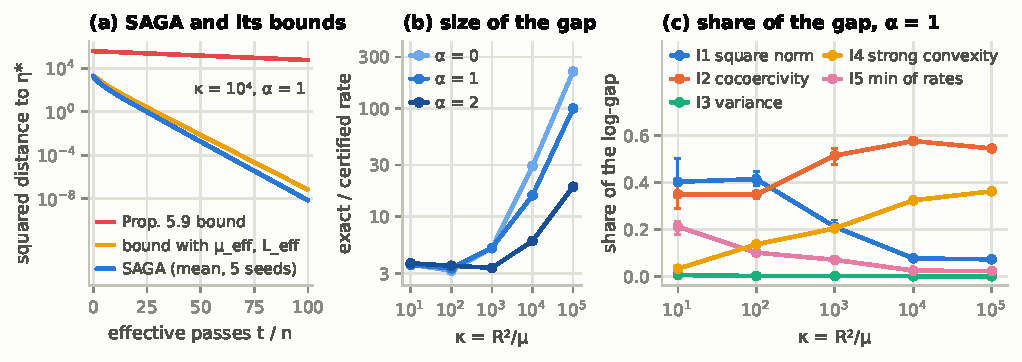
\includegraphics[width=0.97\textwidth]{figR1_classical}
\caption{SAGA with the textbook step on ridge logistic regression ($n=1000$, $d=50$). (a) $\kappa=10^4$, spectrum
$j^{-1}$: certified bound of Proposition~5.9, a-posteriori bound with the effective constants $\muEff,\LEff$ along one
run, and squared distance to the minimizer (mean of five runs). (b) Exact over certified contraction exponent (passes
2--20, five seeds) against $\kappa$, for spectra $j^{-\alpha}$. (c) Share of the logarithmic gap carried by each
inequality ($\alpha=1$; undone in reverse proof order; mean and range over five seeds).}\label{fig:classical}
\end{figure}

\paragraph{Where the proof of SAGA loses} (measured as in Section~\ref{sec:measure}):

\begin{description}[leftmargin=2.3em,labelwidth=2.0em,labelsep=0.3em,itemsep=1pt,topsep=3pt,parsep=0pt,font=\normalfont\bfseries]
\item[(C1)] \emph{The gap.} The exact contraction exponent is $3.2$--$3.7$ times the certified one for
$\kappa\le10^2$ and $19$--$220$ times at $\kappa=10^5$ (Figure~\ref{fig:classical}(b)).
\item[(C2)] \emph{Its anatomy.} For $\kappa\ge10^4$ I2 and I4, which replace a quantity depending on the iterate by a
global constant, carry $77$--$96\%$ of the logarithmic gap; for $\kappa\le10^2$, where the memory term is active, I1
($39$--$44\%$) and I2 ($32$--$37\%$) carry it (Figure~\ref{fig:classical}(c)). The variance step I3 is nearly tight (at
most $0.6\%$ of the gap). In \eqref{eq:saga-repr} the bracket that contains $\LEff$ and $r_{\mathrm{sq}}$ lies in
$[\frac38,1]$ (cocoercivity gives $\LEff\le R^2$), so, through $c_D$, I1 and I2 together contribute at most a factor $8/3$,
whereas $\muEff/\mu$ is bounded only by a condition number; for $\kappa\ge10^4$ the first factor is $2.45$--$2.62$ along
the runs, the second grows with $\kappa$ up to $81$, and their product reproduces $91$--$96\%$ of the speed-ups.
On eight data sets of the two designs of \cite{na2023hessian}, in our port of their public code (leverage scores of
low or high coherence, labels close to noise or as informative as ours), for $\kappa\ge10^4$ I2 and I4 carry
$64$--$98\%$ of the gap and the product reproduces $80$--$97\%$ of the speed-ups, but the size of the gap depends on the
design ($13$ to $198$ at $\kappa=10^5$).
\item[(C3)] \emph{Effective constants explain, they do not certify.} The global strong-convexity constant of ridge
logistic regression is exactly $\lambda$, whatever the data: the loss curvature vanishes at infinity. Near the optimum
$\muEff$ is at least about the smallest eigenvalue of the Hessian at $\etas$, a value that SAGA reaches when its error
aligns with the flattest direction ($\muEff/\mu=9.94$ against $9.86$, $\kappa=10^4$, $\alpha=0$, one run).
Contrary to a heuristic prediction of ours, according to which the estimator noise keeps the error spread over many
directions, at $\kappa=10^4=10n$ ($\alpha\in\{0,1\}$) SAGA keeps and sharpens, as gradient descent does, the alignment
of its initial error with this direction ($89$--$98\%$ of its squared norm at $\theta_0=0$); over nine runs
($\kappa\in\{10^2,10^3,10^4\}$, all $\alpha$, one seed), the prediction holds in exactly the four where the memory term
would be the active one with the local constant in place of $\mu$, $9n\lmin(F''(\etas))/(16R^2)>1$, a dividing line
proposed after the runs.
Rewritten
with $\muEff$ and $\LEff$, the bound of Proposition~5.9 recovers $59$--$96\%$ of the logarithmic gap for $\kappa\ge10^4$
(Figure~\ref{fig:classical}(a)): an a-posteriori reading, not a guarantee.
\end{description}
The same instrument, applied to the Lyapunov proof of loopless Katyusha \cite{kovalev2020dont} in the main report,
finds a smaller gap: on the logistic problems with $\alpha=1$, $\kappa=10^3$ and $10^4$, the one-step contraction
certified by that proof is pessimistic in exponent by a factor $2.8$ and $4.1$, against $5.2$ and $15.7$ for
Proposition~5.9, and its variance bound is loose as I2 is, by the gap between $R^2$ and the curvature met along the run
(tightness $0.15$).

\paragraph{The same anatomy for polar steps.} In \eqref{eq:polar-repr} with $L=\Lop$, the exponent of the exact factor
is, to first order, $(\muPL/\muop)(2-J/\Lop)$ times the certified one, $1/\kop$: the smoothness slack
$2-J/\Lop\in[1,2)$ can gain at most a factor $2$, as I1--I2 at most $8/3$ for SAGA, and the sharpness slack
$\muPL/\muop\in[1,\kop]$ is the only unbounded one, as $\muEff/\mu$ for SAGA. In both, the certified rate is the exact
formula at worst-case values of state-dependent ratios, and beyond a bounded factor a run gains only through the
curvature it meets, measured against the global constant. On least squares, $F=F_\ast+\frac12\tr(E\Sigma E^\top)$ with
$E=W-W_\ast$, the curvature is constant: for $K\ge d$, $p=\lmin(\Sigma)/\tr\Sigma$ and an error with the eigenvectors of $\Sigma$ as
right singular vectors and singular values $\propto1-p$ on the flattest one, $\propto p$ on the others (a ray, invariant up to signs),
the exact factor per step is $(1-2p)^2$ \cite{shulgin2026quadratic}, an exponent about $4$ times the certified one,
and generic starts end close to this ray in the $20\times20$ runs of the theory note, much as the error of SAGA, which
starts mostly on the flattest direction, ends on it at $\kappa=10n$ for $\alpha\in\{0,1\}$ \finding{C3}. A large gap needs a global constant
far below the curvature met near the minimizer, as for logistic and softmax losses (Theorem~\ref{thm:nfl}); we did not
measure the polar step there.

\paragraph{(C4) The analysis cannot repair the worst case.} Within the proof, the best step and Lyapunov weight gain at most
a factor $3$, and at most $4/3$ when $\kappa\ge9n/16$ (the optimum is the step and rate of \cite{hofmann2015variance}).
At $\kappa=10^3$ they gain $17\%$, whereas the observed exponent at the textbook step is $4.5$ times the best
certificate at that step and SAGA still converges at $\gamma R^2=4$, eight times the supremum $\frac12$ of the values of
$\gamma R^2$ the proof admits ($\alpha=1$, three seeds, passes 2--40). Where the memory term binds ($\kappa\le10^2$) the
constants matter more: the best ones multiply the certified exponent by $2.4$--$2.9$, against a measured gap of
$3.2$--$3.7$. The large gaps, which \finding{C2} attributes to the global constants, belong to the regime $\kappa\gg n$.
On $n$ identical components $f_i(\theta)=\frac12(\mu\theta_1^2+R^2\theta_2^2)$, SAGA with any constant step, even one depending on
$\mu$, needs at least $\frac{\kappa-1}4\log\frac1{2\varepsilon}$ iterations to bring $\E\norm{\theta_t}^2$ below $\varepsilon\norm{\theta_0}^2$ from
$\theta_0=(r,r)$, $r\ne0$, since its mean iterate is that of gradient
descent (the order $\kappa$ is that of one-step stationary methods \cite[Theorem~8]{arjevani2016lower}; for steps
depending only on $R^2$ it also follows from \cite{arjevani2016iteration}).

\begin{description}[leftmargin=2.3em,labelwidth=2.0em,labelsep=0.3em,itemsep=1pt,topsep=3pt,parsep=0pt,font=\normalfont\bfseries]
\item[(C5)] \emph{No free lunch for preconditioning.} Proposition~5.9 holds in any fixed quadratic metric $P$ with the
constants $R_P^2,\mu_P$ of Section~\ref{sec:geometry} (as for Bregman-SAGA \cite{dragomir2021fast}), and a metric built
from the data covariance improves them when the loss curvature is bounded below where the predictions lie, as for ridge
regression \cite{yang2014data,gonen2016solving} and, on bounded sets, logistic regression \cite{yang2014data}. For ridge
logistic regression every $P$ has $\kappa_P\ge\kappa$ for these global constants. Yet at $\kappa=10^3$ the statistical
metric $P=\hat\Sigma+\lambda I$ raises the observed exponent per pass from $1.00$ to $1.11$ ($\alpha=1$) and from
$0.61$ to $1.26$ ($\alpha=2$), while the certified bound ranks it below the identity. Along the runs the metric moves
the slack of the proof from cocoercivity to strong convexity: for $\alpha=1$ the tightness ratios of I2 and I4 in the
metric, $\LEff/R_P^2$ and $\mu_P/\muEff$ (computed in the norm of $P$), go from $0.13$ to $0.33$ and from $0.42$ to
$0.017$, the trade that Theorem~\ref{thm:nfl} below makes general for the global constants. The gain is a property of
the trajectory: on these instances only local constants at the optimum account for it, heuristically. On eight data
sets of the designs of \cite{na2023hessian} (feature covariance of condition number $2500$; three of low, five of high
coherence) with labels close to pure noise, hence nearly homogeneous curvatures at the optimum, a rigorous bound on
$R_P^2/\muEff$ along the run, through ridge leverage scores and the smallest per-sample curvature, is informative: it
is $1.3$--$2.5$ times the measured value and below $\kappa$ on seven of them.
\end{description}

\begin{theorem}[no free lunch, for every norm]\label{thm:nfl}
Consider (GLM) and assume that there is a sequence $W_t$ with $\max_i\nop{\nabla^2\ell_i(W_tx_i)}\to0$ (logistic and
softmax losses with nonzero $x_i$: $W_t=tW_1$ for almost every $W_1$). Let $N$ be any norm on $\R^{K\times d}$ and
$c_N=\max_{\nF\Delta=1}N(\Delta)$. Then $\mu_N(F)=\lambda/c_N^2$ and $L_N(g)\ge L_F(g)/c_N^2$ for every convex $C^2$
function $g$. Consequently $\kappa_N(F)\ge\kF(F)$ and $L_N(f_i)/\mu_N(F)\ge L_F(f_i)/\mu_F(F)=(c_i\norm{x_i}^2+\lambda)/\lambda$
for every $i$.
\end{theorem}
\begin{proof}
For all $W,\Delta$, $D^2F(W)[\Delta,\Delta]\ge\lambda\nF\Delta^2\ge(\lambda/c_N^2)N(\Delta)^2$. At a maximizer
$\Delta_0$ of $N/\nF\cdot$, $D^2F(W_t)[\Delta_0,\Delta_0]\le\max_i\nop{\nabla^2\ell_i(W_tx_i)}\frac1n\sum_i\norm{\Delta_0x_i}^2
+\lambda\nF{\Delta_0}^2\to\lambda\nF{\Delta_0}^2=(\lambda/c_N^2)N(\Delta_0)^2$, so $\mu_N(F)=\lambda/c_N^2$; the same
computation with $N=\nF\cdot$ gives $\mu_F(F)=\lambda$. For a convex $g$, $D^2g[\Delta,\Delta]/N(\Delta)^2\ge
D^2g[\Delta,\Delta]/(c_N^2\nF\Delta^2)$; take suprema. Finally $L_F(f_i)=c_i\norm{x_i}^2+\lambda$, approached in the
directions $ex_i^\top/\norm{x_i}$, $e$ a top eigenvector of $\nabla^2\ell_i(Wx_i)$, as $\lmax(\nabla^2\ell_i(Wx_i))\to c_i$.
\end{proof}

It covers the spectral norm and its preconditioned versions, the $\ell_\infty$ norm of sign descent and
Kronecker-factored metrics; for $K=1$
and Euclidean metrics it is \finding{C5}, and functions that no linear preconditioner improves exist in every dimension
\cite[Proposition~7]{hird2025quantifying}. The mechanism is that the curvature floor of a ridge model is isotropic and
attained in the limit along $W_t$: a norm can only trade smoothness against strong convexity, and any advantage of
a step in another norm on such problems is a property of the trajectory. The hypothesis on the losses is needed: for
ridge least squares the norm $\nF{\Delta\Sigma^{1/2}}$, $\Sigma$ the Hessian, has condition number one. The spectral
geometry even has its own cost: $\kop\ge\min(K,d)$ for every $F$, the matrix form of a folklore fact on
$\ell_\infty$ \cite{sidford2018coordinate}.

\begin{figure}[t]
\centering
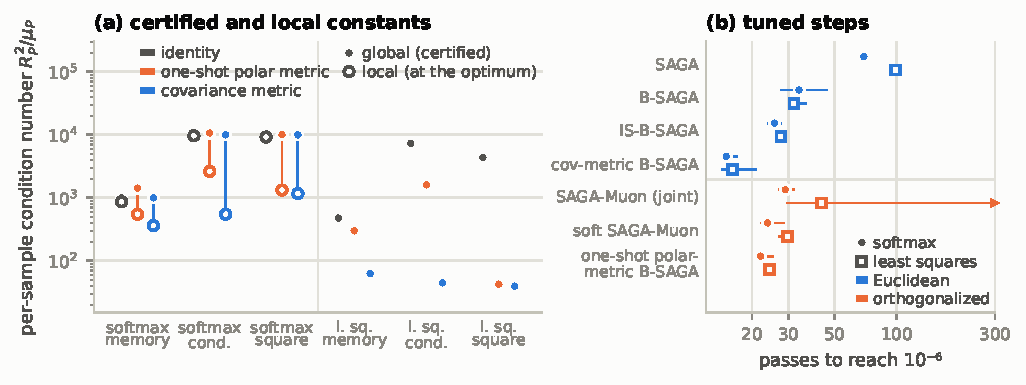
\includegraphics[width=0.97\textwidth]{figP2_geometry}
\caption{Geometry of Muon-type steps on the six instances of Section~\ref{sec:experiments}. (a) Per-sample condition
number $R_P^2/\mu_P$ of SAGA in three fixed metrics: identity, one-shot polar metric and feature-covariance metric (best
over $f$). Filled: global constants, which a proof can use; open: with $\mu_P$ at the optimum (global $R_P^2$), each at its
own best $f$.
For least squares the two coincide (constant Hessian, one marker). (b) Passes to $10^{-6}$ at tuned steps on the two
non-square conditioning-limited instances (median and range over ten seeds; arrow: a seed misses the target). B-SAGA:
damped innovation; IS: importance sampling; cov-metric: feature-covariance metric.}\label{fig:geometry}
\end{figure}

\paragraph{What it means for Muon-type steps.} Two experiments carry Theorem~\ref{thm:nfl} to the benchmark.

\begin{description}[leftmargin=2.3em,labelwidth=2.0em,labelsep=0.3em,itemsep=1pt,topsep=3pt,parsep=0pt,font=\normalfont\bfseries]
\item[(M4)] \emph{Certified constants: a frozen polar metric certifies a gain only where the theorem does not apply.} If
the map $\omega\mapsto\omega C$ of Section~\ref{sec:geometry} is computed once, the method is SAGA in a fixed metric,
and Proposition~5.9 holds with $R_P^2,\mu_P$ in place of $R^2,\mu$ \finding{C5}. On softmax, none of the metrics tested improves the
global constant, as Theorem~\ref{thm:nfl} requires (Figure~\ref{fig:geometry}(a): the best ratio to the Euclidean one is
exactly $1$, reached only by the identity), while the local constants are up to $17.5$ times smaller than for the
identity (covariance metric, conditioning-limited softmax: $551$ against $9659$). On least squares, where the
loss curvature does not vanish, the certified constant improves by a factor $1.6$ to $103$ in the polar metric ($7.6$ to $163$ in the covariance metric); on the square least-squares
instance, where the polar factor of the gradient is close to the Newton direction \cite{shulgin2026quadratic},
$R_P^2/\mu_P=42$ against $R^2/\mu=4364$, and this ``one-shot polar-metric SAGA'' needs $13.3$ passes (SAGA $27.1$,
covariance metric $13.1$).
\item[(M3)] \emph{Observed speed: orthogonalization buys a trajectory effect that Euclidean devices reproduce.} Where
the conditioning limits (the two non-square instances: softmax / least squares), SAGA needs $69.5$ / $98.7$ passes, the
orthogonalized methods $22.1$--$29.0$ / $24.4$--$43.5$ (joint SAGA-Muon, its soft version, damped SAGA in a polar
metric frozen once; one seed of the joint method misses the target on least squares), and the Euclidean devices $15.1$--$33.8$ / $16.1$--$31.9$ (damped SAGA, with importance sampling,
in the feature-covariance metric) (Figure~\ref{fig:geometry}(b)). Over three draws of the data, the best method recomputing the polar factor
needs $0.20$--$0.37$ of the passes of SAGA and $0.78$--$1.08$ of those of the best Euclidean method without
preconditioner; the covariance metric is the best method on least squares for every draw, and on softmax for one draw
of three (undamped; the damped version was not rerun). Where the memory limits, the best family of every class
(Euclidean, orthogonalized, fixed metric) needs $16$--$18$ (softmax) and $17$--$21$ passes (least squares) to
$10^{-9}$, near the memory ceiling of SAGA: no bound on its expected Lyapunov function certifies better than $e^{-1}$
per pass, since stale entries keep their error.
\end{description}

\subsection{Finding 2: through the polar map, variance reduction acts on the fixed point}\label{sec:f2}

The polar map breaks the first property of the SAGA estimator, unbiasedness ($\E\,\polar(G+\xi)\ne\polar(G)$ in
general), and noise can move the limit (Theorem~\ref{thm:smd}); it keeps the second, an error that vanishes at the
minimizer, and the minimizer is again the only fixed point (Proposition~\ref{prop:comp}(c)). With the objects of
Section~\ref{sec:noisemethod},
$\arg\min\psi_\xi=-\Med(\xi)$ is nonempty, convex and compact; it contains every zero of $\Phi_\xi$, and consists of
zeros of $\Phi_\xi$ where $G+\xi$ has full rank almost surely (otherwise the mean field may have no zero: for the
scalar law $\Prob(\xi=1)=0.4$, $\Prob(\xi=-1)=0.6$, the minimizer of $\psi_\xi$ is $g=1$ and $\abs{\Phi_\xi}\ge0.2$
everywhere).

\begin{theorem}[stochastic polar steps are stochastic mirror descent]\label{thm:smd}
Let $F$ satisfy $0<\muop\le\Lop<\infty$, let $\xi_t$ be i.i.d.\ copies of $\xi$ independent of the past, $\eta_t\ge0$
deterministic lengths, and $W_{t+1}=W_t-\eta_t\,\polar(\nabla F(W_t)+\xi_t)$, $G_t=\nabla F(W_t)$. For every
$G^\dagger\in\arg\min\psi_\xi$, with $W^\dagger=\nabla F^\ast(G^\dagger)$ and $D_F$ the Bregman divergence of $F$:
\begin{enumerate}[label=(\alph*),itemsep=0pt,topsep=2pt]
\item $\E[D_F(W_{t+1},W^\dagger)\mid W_t]\le D_F(W_t,W^\dagger)-\eta_t(\psi_\xi(G_t)-\min\psi_\xi)+\frac{\Lop}2\eta_t^2$,
hence $\E\,\psi_\xi(\bar G_T)-\min\psi_\xi\le\big(D_F(W_0,W^\dagger)+\frac{\Lop}2\sum_{t<T}\eta_t^2\big)/\sum_{t<T}\eta_t$
with $\bar G_T=\sum_{t<T}\eta_tG_t/\sum_{t<T}\eta_t$, whatever the lengths;
\item if $\sum_t\eta_t=\infty$ and $\sum_t\eta_t^2<\infty$, $G_t$ converges almost surely to a point of $-\Med(\xi)$;
\item hence, for such lengths, almost surely: $W_t\to W_\ast$ if $\Med(\xi)=\{0\}$, and if $0\notin\Med(\xi)$ then
$\lim_tF(W_t)-F_\ast\ge\min_{C\in\Med(\xi)}\nnuc C^2/(2\Lop)>0$.
\end{enumerate}
\end{theorem}
\begin{proof}[Proof sketch]
$\nabla F$ is a bijection with inverse $\nabla F^\ast$, and $W^+=W-\eta O$ reads $\nabla F^\ast(G^+)=\nabla F^\ast(G)-\eta
O$: one step of mirror descent in the space of gradients, with mirror map $F^\ast$ (as in \cite{maddison2021dual}, there for smooth maps of the gradient). The
three-point identity gives
$D_{F^\ast}(G^\dagger,G_{t+1})=D_{F^\ast}(G^\dagger,G_t)-\eta_t\inner{O_t}{G_t-G^\dagger}+D_{F^\ast}(G_t,G_{t+1})$, with
$O_t=\polar(G_t+\xi_t)$; moreover $D_{F^\ast}(G',G)=D_F(W,W')$ and $D_F(W_{t+1},W_t)\le\frac{\Lop}2\nop{W_{t+1}-W_t}^2\le
\frac{\Lop}2\eta_t^2$. Conditionally on $W_t$, $\E\inner{O_t}{G_t-G^\dagger}=\inner{\Phi_\xi(G_t)}{G_t-G^\dagger}\ge
\psi_\xi(G_t)-\psi_\xi(G^\dagger)$, because $\Phi_\xi(G_t)\in\partial\psi_\xi(G_t)$. This is (a); summing and convexity
give the averaged bound. (b): by the Robbins--Siegmund lemma $D_F(W_t,W^\dagger)$ converges and
$\sum_t\eta_t(\psi_\xi(G_t)-\min\psi_\xi)<\infty$ almost surely; $\psi_\xi$ is coercive, a cluster point of $G_t$ is a
minimizer, and the convergence of $D_F(W_t,W')$ for a countable dense set of minimizers gives that of the whole
sequence. (c): the dual-norm Polyak--\L{}ojasiewicz inequalities
$2\muop(F(W)-F_\ast)\le\nnuc{\nabla F(W)}^2\le2\Lop(F(W)-F_\ast)$ \cite{kakade2012regularization,balles2020geometry}.
\end{proof}

The theorem replaces the usual condition $\E\xi=0$ by $\Med(\xi)=\{0\}$; otherwise the limit gradient, a point of
$-\Med(\xi)$, is an \emph{offset}, and no schedule of this class removes it: the set of possible limits does not depend
on the lengths. Its ingredients are published, and so are its scalar and coordinatewise analogues: sign methods drive a median of the stochastic
gradient to zero \cite{chen2020distributed}, and normalized steps on a location problem estimate the geometric median
\cite{cardot2013efficient}. The statement for polar steps was not found.

\begin{proposition}[when is there an offset?]\label{prop:comp}
(a) If $\xi$ and $-\xi$ have the same law, $0\in\Med(\xi)$, and $\Med(\xi)=\{0\}$ if moreover $0$ is in the support
of $\xi$.
(b) If $\xi$ is integrable and $\E\xi=0$, every $C\in\Med(\xi)$ has $\nnuc C\le\E\nnuc\xi$, so the limit of
Theorem~\ref{thm:smd} has $F(W^\dagger)-F_\ast\le(\E\nnuc\xi)^2/(2\muop)$.
(c) For a SAGA or SVRG estimator, the stochastic gradient at $W_\ast$, with its memory (table or reference point) also
at $W_\ast$, is $0$ for every index: a Dirac mass, whose median is its mean. Such estimators have a fixed point
without offset (a state, iterate and memory, that no index moves), and it is the only one.
(d) (Batch one on least squares.) Let $g_j(W)=(Wx_j-y_j)x_j^\top$, $x_j\ne0$, $j$ uniform in $\{1,\dots,n\}$. The
batch-one polar step is the stochastic subgradient method on $\Lambda(W)=\frac1n\sum_i\norm{Wx_i-y_i}/\norm{x_i}$; with
deterministic lengths, $\sum_t\eta_t=\infty$, $\sum_t\eta_t^2<\infty$, it converges almost surely to a minimizer of this
weighted least-distances objective, in general not the least-squares solution.
\end{proposition}
\begin{proof}
(a) $\psi_\xi$ is even (symmetric law) and convex, hence minimal at $0$; and
$\psi_\xi(G)-\psi_\xi(0)=\frac12\E[\nnuc{\xi+G}+\nnuc{\xi-G}-2\nnuc\xi]$ has a nonnegative integrand, at least
$2\nnuc G-2\nnuc\xi>0$ on $\{\nnuc\xi<\nnuc G\}$. (b) $C=\E[C-\xi]$ gives $\nnuc C\le\E\nnuc{\xi-C}\le\E\nnuc\xi$
(Jensen, then minimality of $C$ against $0$); then Theorem~\ref{thm:smd} and the inequality $F-F_\ast\le
\nnuc{\nabla F}^2/(2\muop)$. (c) With $z_i=f_i'(W_\ast)$, $\omega_j=f_j'(W_\ast)-z_j+\bar z=\nabla F(W_\ast)=0$ and
$\polar(0)=0$; conversely a table that no index changes satisfies $z_i=f_i'(W)$, hence $\omega_j=\nabla F(W)$ for every
$j$, which vanishes only at $W_\ast$. (d) For $r=Wx-y\ne0$, $\polar(rx^\top)=rx^\top/(\norm r\norm x)=\nabla_W\norm{Wx-y}/\norm x$
\cite[Lemma~H.1]{li2026implicit}, and $\polar(0)=0$ is a subgradient; the rest is the stochastic subgradient method for a
convex Lipschitz function.
\end{proof}

Item (a) parallels the unimodal symmetric-noise condition under which signSGD converges \cite{bernstein2019majority};
(b) is the classical inequality between mean and median, in a normed space; (c) identifies a fixed point, not its
attraction. For $K=1$ the limit in (d) is classical (sign-error algorithms minimize a mean absolute error), for $d=1$ it
is the geometric median of the $y_i/x_i$ \cite{cardot2013efficient}, and for coordinatewise sign descent at batch size
one non-convergence for every step-size sequence is proved in \cite{karimireddy2019error} (Theorem~I) when all data
points share a sign pattern, and on a separable data set batch-one spectral descent with reshuffling has a limit
direction other than the full-batch one \cite[Theorem~4.10]{li2026implicit}; for $K,d\ge2$ (d) was not found. With lengths proportional to the sampled gradient,
$\eta_t=\nnuc{g_j(W_t)}/(t+t_0)$, the step is $g_j(W_t)/(t+t_0)$, plain stochastic gradient descent, which converges
to the least-squares solution: the hypothesis of deterministic lengths is needed.

\begin{proposition}[size of the offset for minibatches; formal]\label{prop:offset}
Let $\xi_b$ be the mean of $b$ i.i.d.\ centred matrices with i.i.d.\ entries of variance $\sigma^2$ and third
cumulant $\kappa_3$, with a non-lattice law. A one-term Edgeworth expansion gives, for the minimizer $G_b^\dagger$ of
$\psi_{\xi_b}$,
\begin{equation}\label{eq:offset}
G_b^\dagger=\frac{\kappa_3}{6\sigma^2b}\cdot\frac{a_{K,d}}{c_{K,d}}\;\ones\ones^\top+o\Big(\frac1b\Big),\qquad
a_{K,d}=-\E\big[\polar(Z)_{11}(Z_{11}^3-3Z_{11})\big],\quad c_{K,d}=\frac{\E\nnuc Z}{Kd},
\end{equation}
with $Z$ a standard Gaussian $K\times d$ matrix: in every entry, the scalar offset $\kappa_3/(6\sigma^2b)$ of the
median of a mean (Cornish--Fisher \cite{cornish1938moments}) times $a_{K,d}/c_{K,d}$.
\end{proposition}

Since $\polar$ is homogeneous of degree $0$, $\Phi_{\xi_b}(0)=\E\polar(\sqrt b\,\xi_b)$; the Edgeworth correction of the law
of $\sqrt b\,\xi_b$ gives $\Phi_{\xi_b}(0)=\mathcal T/\sqrt b+O(b^{-3/2})$ for a third-cumulant term $\mathcal T$, the
derivative of the mean field at $0$ is $\sqrt b\,c_{K,d}/\sigma$ to first order (the Gaussian response of
\cite{xie2026muon,chen2026when}), and solving $\Phi_{\xi_b}(G)=0$ to first order gives \eqref{eq:offset}. The expansion
is formal (an Edgeworth expansion against a discontinuous map), but its predictions are parameter-free. What matters is the skewness of the \emph{gradient} noise: with symmetric inputs
independent of the residuals the offset is zero, and an intercept suffices to create one. The constant
$a_{K,d}/c_{K,d}$, symmetric in $(K,d)$, is numerically of order $1/\max(K,d)$: it equals $3/(d+2)$ exactly for $K=1$
(Gaussian integration by parts), and $\max(K,d)\,a_{K,d}/c_{K,d}$ lies between $1.4$ and $2.8$ for ten sizes with
$2\le K\le d$, from $2\times2$ to $32\times32$ and $16\times64$ (quadrature for $2\times2$ and $2\times3$, Monte Carlo
otherwise, relative standard errors below $3\%$). Per entry, the offset of the polar step is thus smaller than that of
sign descent by a factor of order $\max(K,d)$, and its objective gap is of order $1/b^2$. For Muon itself, in dimension
one with the Newton--Schulz map and momentum, \cite{do2026muon} prove non-convergence for bounded data with a nonzero
third central moment, for almost all batch sizes (Theorem~1.3), and show that every limit is a zero of the mean field
(Proposition~6.2).

\begin{figure}[t]
\centering
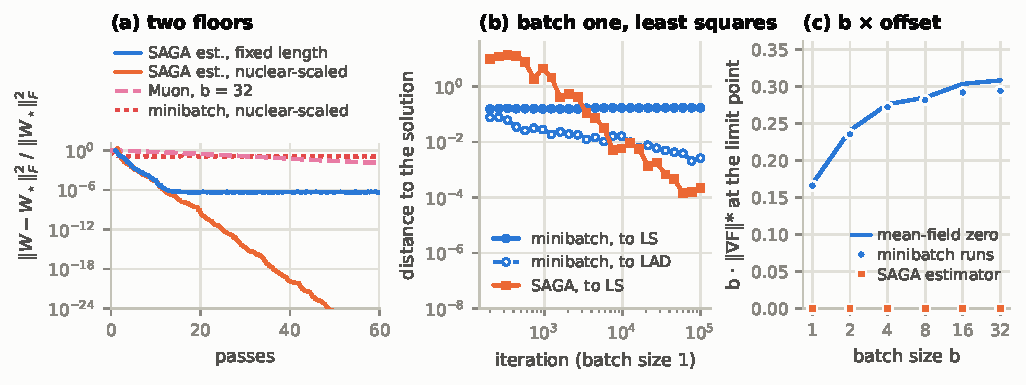
\includegraphics[width=0.97\textwidth]{figP3_noise}
\caption{What a finite-sum estimator changes inside polar steps. (a) Softmax, memory-limited instance, one seed,
constant parameters (SAGA estimator with the fixed length $10^{-2}$ or the nuclear-scaled one; Muon with
$\mathrm{lr}=10^{-2}$ and the minibatch gradient with the nuclear-scaled length, both with $b=32$): relative squared
distance to the minimizer. (b) Unregularized finite-sum least squares with an intercept and skewed residuals ($n=2000$,
$K=2$, $d=3$), batch one, lengths $\eta_t=0.3\,(1+t/200)^{-3/4}$ from $W_0=0$: with the minibatch gradient the iterate,
averaged over $(t/2,t]$ and over $32$ runs, converges to the least-distances solution $W_{\mathrm{LAD}}$ of
Proposition~\ref{prop:comp}(d); with the SAGA estimator, after an excursion while its table (initialized at $W_0$) is
stale, to the least-squares solution $W_{\mathrm{LS}}$ (one pass: $2000$ iterations). (c) Same problem: batch size times
the nuclear norm of the limit gradient, for the zeros of the mean field (line), runs with decreasing lengths
(dots; same averaging, $64$ runs) and the SAGA estimator with the nuclear-scaled length (squares, at rounding
level).}\label{fig:noise}
\end{figure}

\paragraph{Numerical checks.} For $2\times3$ matrices with entries $\mathrm{Exp}(1)-1$, \eqref{eq:offset} predicts
$b\,\nnuc{G_b^\dagger}\to0.464$; the zero of the mean field computed from $1.5\cdot10^6$ exactly sampled batch means
gives $0.450$--$0.498$ for $b=2,\dots,256$, the extremes at $b=2$ and $b=256$ (higher-order terms; Monte-Carlo
error of the root). On the finite sum of Figure~\ref{fig:noise}(b)--(c)
($\nF{W_{\mathrm{LAD}}-W_{\mathrm{LS}}}=0.170$; rank-one per-sample gradients, so \eqref{eq:offset} does not apply as
such), averaged batch-one polar steps with decreasing lengths end $2.6\cdot10^{-3}$ from $W_{\mathrm{LAD}}$ and $0.169$
from $W_{\mathrm{LS}}$, the SAGA estimator with the same lengths $2.1\cdot10^{-4}$ from $W_{\mathrm{LS}}$; for $b\le32$
the runs end within $5\%$ of the zero of the mean field $W\mapsto\E\,\polar(\nabla F_B(W))$ ($B$ the batch; exact
for $b=1$, Monte Carlo otherwise), $b$ times the offset
rises from $0.17$ to a plateau near $0.3$, and the SAGA estimator with the nuclear-scaled length ends at rounding level
(gradient norm below $2.4\cdot10^{-15}$).

\paragraph{Three obstructions to precision, and what acts on each.} A polar step with stochastic gradients meets the
length floor of a fixed length, the fluctuations of a constant step, and, with decreasing lengths, the median offset
(Theorem~\ref{thm:smd}; Proposition~\ref{prop:comp}(d)). Figure~\ref{fig:noise}(b)--(c) shows the offset and its removal by the SAGA estimator; the runs
with constant parameters separate the other two \finding{M1}, and \finding{M2} identifies the method at batch one.

\begin{description}[leftmargin=2.3em,labelwidth=2.0em,labelsep=0.3em,itemsep=1pt,topsep=3pt,parsep=0pt,font=\normalfont\bfseries]
\item[(M1)] \emph{Length floor and noise floor} (Figure~\ref{fig:noise}(a)). Polar steps of fixed length stall at a
floor \cite{lau2025polargrad,jawanpuria2026constant}; as in \cite[Lemma~4]{jawanpuria2026constant}, with a constant spectral length $\eta$,
$\max(F(W_t),F(W_{t+1}))-F_\ast\ge\muop\eta^2/8$ whenever the step is nonzero. Variance reduction does not remove
it: with the SAGA estimator and a fixed length $\eta$ the iterates settle at an absolute squared distance $3.8\,\eta^2$
(softmax) or $6.0\,\eta^2$ (least squares), quadratic in the length, whereas the floor of minibatch Muon is linear in its
learning rate. A nuclear-scaled length removes the length floor but not the noise: with the minibatch gradient ($b=32$)
the runs settle at a relative squared distance $1.2\cdot10^{-1}$ (softmax) or $4.8\cdot10^{-2}$ (least squares), and a
momentum-based buffer (as in MARS-M \cite{liu2025marsm}) keeps a noise floor at constant parameters whatever the length.
Only a finite-sum estimator with a step that vanishes with it (nuclear-scaled or clipped length; on least squares also
the soft map with a fixed $\epsilon$) reaches rounding precision, as Proposition~\ref{prop:comp}(c) leads one to expect.
\item[(M2)] \emph{At batch size one, the nuclear-scaled polar step of SAGA is MISO in disguise.} The predictable part $m$ is the gradient of an isotropic quadratic, the orthogonalized
matrix is dominated by the rank-one innovation (exact one-step expectations give the estimator a nuclear rank
$\nnuc\omega^2/\nF\omega^2$ of $1.07$, median over the recorded states of the softmax memory-limited instance), and the
nuclear-scaled step drives $m$ to zero; the method that keeps $m=0$ exactly is MISO (Section~\ref{sec:experiments}).
With the same sampled indices the traces follow each other (extended report, Figure~2(b)): the joint SAGA-Muon needs the passes of MISO where MISO
converges ($11.8$ against $11.9$, medians of three seeds, softmax with $\kappa=n$; SAGA at its textbook step: $20.2$)
and fails where MISO fails ($\kappa\gg n$). It is not a spectral method.
\end{description}

\section{Discussion}\label{sec:discussion}

\subsection{From SAGA to Muon: the link, property by property}\label{sec:link}

\begin{table}[t]
\caption{The two properties behind the rate of SAGA, and what becomes of them in Muon-type steps.}\label{tab:link}
\centering\footnotesize
\renewcommand{\arraystretch}{1.1}
\begin{tabularx}{\textwidth}{@{}>{\raggedright\arraybackslash}p{0.2\textwidth}YYY@{}}
\toprule
Ingredient of SAGA & In the SAGA study & In Muon-type steps & Consequence \\
\midrule
\emph{Geometry}: global constants $\mu,R^2$ certify the rate. &
The proof loses at I2 and I4, where the curvature met ($\muEff$ up to $81\mu$) is replaced by $\mu$ and $R^2$
\finding{C2}, \finding{C3}; no fixed metric improves $\kappa$ on logistic losses \finding{C5}. &
The nuclear-scaled step has the same exact anatomy \eqref{eq:polar-repr}; no norm, the spectral one included, improves
the worst case when the loss curvature vanishes (Theorem~\ref{thm:nfl}). &
Finding 1: without a floor on the loss curvature, a change of norm buys only trajectory properties, which Euclidean devices
reproduce \finding{M3}; with one, certified gains, as on least squares \finding{M4}. \\
\emph{Estimator, first}: unbiased, so the mean step is the gradient step. &
Exact in a linear step. &
Lost: the mean step is a mirror subgradient step on the noise-smoothed nuclear norm (Theorem~\ref{thm:smd}). &
Finding 2: the limit gradient is minus a nuclear median of the noise, formally of order $1/b$ (Proposition~\ref{prop:offset}). \\
\emph{Estimator, second}: the error vanishes at the minimizer. &
Removes the variance term: linear rate with a constant step. &
Kept: the minimizer is the only fixed point (Proposition~\ref{prop:comp}(c)). &
Finding 2: with a step that vanishes with the estimator, rounding precision \finding{M1}; at batch one, MISO \finding{M2}. \\
\emph{Tool}: exact one-step expectations over the $n$ indices. &
Measures each inequality of the proof \finding{C1}--\finding{C3}. &
The same enumeration, although the step is nonlinear in the estimator. &
Exact mean steps: \finding{M2} and the zeros of the mean field at batch one. \\
\bottomrule
\end{tabularx}
\end{table}

Table~\ref{tab:link} sums up the link, negative for changes of norm where the loss curvature vanishes and positive, but
not Euclidean, for the estimator. It is one of tools, questions and the mechanism of Section~\ref{sec:f2}, not a
reduction: when
the polar factor is recomputed at every step the proof of SAGA does not apply and we have no convergence proof, and the
results on noise without a finite sum (Theorem~\ref{thm:smd}, Proposition~\ref{prop:offset}) owe nothing to SAGA but the
question. Other devices did not transfer (an orthogonalized loopless-SVRG estimator, a spectral step in loopless
Katyusha \cite{kovalev2020dont}, a refreshed polar metric; extended report, Section~3.2).

\subsection{Relation to prior work}\label{sec:prior}

Beyond Table~\ref{tab:sota}: finite-sum estimators in fixed-length polar steps \cite{li2026implicit}, in general norms
\cite{allenzhu2018katyusha} and with a preconditioner computed once \cite{yang2014data} are published; a SAGA table in the
nuclear-scaled polar step at a constant step size, the reading \finding{M2} and a frozen metric taken from the polar
decomposition of one gradient were not found by the check of 12 November 2026. The full-batch dynamics on least squares
\cite{shulgin2026quadratic,vasudeva2025muon} and the regime of low signal-to-noise ratio
\cite{xie2026muon,chen2026when,paquette2026phases} are largely published and not developed here.

\subsection{Limitations}

Everything is for strongly convex objectives and synthetic data of moderate size; the shares of \finding{C2} depend on
the order in which the inequalities are undone; \finding{M3} rests on one to three data draws per instance and counts
gradients, not factorizations. Theorem~\ref{thm:nfl} concerns global constants, not the local ones where the gains are.
Theorem~\ref{thm:smd} assumes additive noise, deterministic lengths and no momentum (for finite-sum minibatches the law
of the noise depends on the iterate; only batch one on least squares is treated); Proposition~\ref{prop:offset} is
formal, and the $1/\max(K,d)$ scaling of its constant is numerical (exact for $\min(K,d)=1$).

\subsection{Conclusion}

The textbook proof of SAGA has the right worst-case order but, measured along trajectories, loses where it replaces the
curvature met along the run by global constants (by large factors when $\kappa\gg n$), as does the exact formula of the nuclear-scaled polar step, and no
fixed change of geometry, Euclidean or spectral, repairs the worst case on ridge logistic and softmax models. For
Muon-type steps, finite-sum variance reduction matters less for speed, where Euclidean devices do as well,
than for precision: with additive noise and deterministic decreasing lengths, polar steps converge to a point where the
gradient is minus a nuclear median of the noise, whereas a finite-sum estimator makes the minimizer the only fixed
point.

\paragraph{Reproducibility and use of AI tools.} Main report \nolinkurl{report/main.pdf}, extended report
\nolinkurl{muon/report_spectral_muon_new.pdf}, theory notes \nolinkurl{muon/notes_spectral_theory.pdf} and
\nolinkurl{muon/notes_theory.md}, logs \nolinkurl{muon/findings.md} and \nolinkurl{muon/results/digest.md}.
All numbers come from scripts in \nolinkurl{experiments/}, \nolinkurl{muon/experiments/} (for (M1)--(M4):
\texttt{exp\_M3}; \texttt{exp\_M6}, \texttt{exp\_M2}; \texttt{exp\_M1}, \texttt{exp\_M8}; \texttt{exp\_M7}, \texttt{exp\_M1}) and
\nolinkurl{muon/theory_checks/}; the figures from \nolinkurl{muon/report_figures/}. A
large language model (Claude, Anthropic) was used under the authors' supervision to derive and check the statements,
write the scripts and run adversarial reviews of the mathematics and the literature (theorem numbers of preprints are
those read then).

{\footnotesize\setlength{\columnsep}{1.6em}
\begin{multicols}{2}[\section*{References}]
\sloppy
\bibliographystyle{abbrv}
\bibliography{paper_saga_to_muon}
\end{multicols}
}

\end{document}
